\section{Implementação em C}
Nesta seção, implementaram-se, na linguagem C, os algoritmos em tópico a fim de analisar os impactos no desempenho quando executado um algoritmo em uma linguagem compilada, tal como o C.
Após visto o comportamento dos algoritmos em Python, uma linguagem interpretada, percebe-se que, mesmo para vetores pequenos, o tempo gasto para ordená-los é significativo. Este problema pode acarretar em diversos...

Quando implementados utilizando a linguagem C, contudo, nota-se uma considerável redução na duração dos testes, uma vez que, em razão do C ser uma linguagem compilada, as malhas de repetição tendem a ser mais eficientes.
Ademais, ao utilizar a linguagem C, há um maior controle na forma como o código será executado, devido ao C ser uma linguagem com um nível mais baixo e tipada, em outras palavras, há uma possibilidade de otimizar o código de maneira mais eficaz.


Dessa forma, serão analisados os desempenhos de alguns dos algoritmos já implementados em Python, mas, desta vez, estes serão escritos na linguagem C.
A fim de realizar o testes, os algoritmos foram implementados na linguagem C, utilizando, como referência, os códigos já escritos em Python. Sendo assim, tendo em vista que os códigos utilizandos em C não foram otimizados e nem modificados de forma a deixá-los mais lentos, ter-se-á uma comparação equânime.
Além disso, as funções foram invocadas no Python visando criar os gráficos dos resultados.

Por fim, é necessário ressaltar que foram realizados somentes testes visando analisar o comportamento dos algoritmos em C quando estes são submetidos a listas com tamanhos variáveis, ou seja, o segundo teste não será executado, pois será obtido resultados similares ao anterior.

\newpage
\subsection{Resultados}
A seguir, serão analisados os resultados encontrados, assim como no primeiro teste, realizando a execução dos algoritmos implementados em C e, para fins comparativos, do algoritmo contagem cuja realização foi feita na linguagem principal.
\begin{figure}[h]
    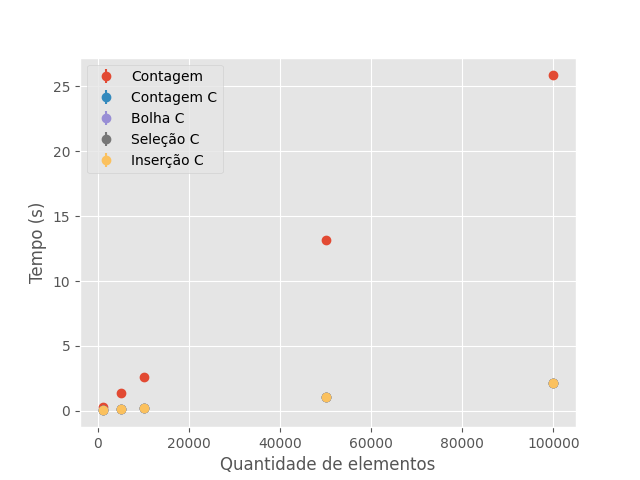
\includegraphics[width=8cm]{c sizes.png}
    \caption{Gráfico ilustrando o tempo médio de execução dos algoritmos implementados em C comparado ao do contagem, implementado em Python.}
\end{figure}
\begin{table}[h]
    \centering
    \begin{tabular}{llllll}
        \textbf{Tamanho} & \textbf{Contagem Py} & \textbf{Contagem} & \textbf{Bolha} & \textbf{Seleção} & \textbf{Inserção} \\
        1000 & 0.2798 & 0.0221 & 0.0222 & 0.0219 & 0.0220 \\
        5000 & 1.3991 & 0.1099 & 0.1088 & 0.1091 & 0.1064 \\
        10000 & 2.5873 & 0.2151 & 0.2136 & 0.2151 & 0.2147 \\
        50000 & 13.1278 & 1.0672 & 1.0653 & 1.0638 & 1.0609 \\
        100000 & 25.9120 & 2.1320 & 2.1423 & 2.1244 & 2.1281 \\
    \end{tabular}
    \caption{Tempos de execução dos algoritmos de ordenação (em segundos) para diferentes tamanhos de lista}
    \label{tab:tempos_ordenacao}
\end{table}

Abaixo, encontram-se os desvios-padrões de cada algoritmo com os respectivos tamanhos das listas ordenadas.
\begin{table}[h]
    \centering
    \begin{tabular}{llllll}
        \textbf{Tamanho} & \textbf{Contagem Py} & \textbf{Contagem} & \textbf{Bolha} & \textbf{Seleção} & \textbf{Inserção} \\

        1000 & 0.001368 & 0.000001 & 0.000002 & 0.0000001 & 0.0000004 \\
        5000 & 0.041076 & 0.000023 & 0.000003 & 0.000002 & 0.000003 \\
        10000 & 0.000821 & 0.000006 & 0.000007 & 0.000017 & 0.000010 \\
        50000 & 0.068934 & 0.000065 & 0.000035 & 0.000022 & 0.000053 \\
        100000 & 0.019201 & 0.000073 & 0.002216 & 0.000139 & 0.000056 \\
    \end{tabular}
    \caption{Desvios padrão dos tempos de execução dos algoritmos de ordenação (em segundos) para diferentes tamanhos de lista}
    \label{tab:desvios_ordenacao}
\end{table}

%TODO melhorar este texto
De início, nota-se que o comportamento dos algoritmos não é modificado, isto é, permaneceram inalteradas, quando implementados em C, características como o uma maior oscilação (maior desvio-padrão) no tempo dos algoritmos que variavam dependendo da taxa de ordenação inicial.
Assim, o comportamento esperado dos algoritmos ainda é visível, independente da linguagem utilizada na implementação.


Perceptivelmente, o ganho de desempenho dos algoritmos implementados em C mostrou-se singificativo; mesmo os mais lentos quando implementados em Python, como o bolha, obtiveram uma performance superior ao contagem da linguagem inicial.
Por outro lado, não houve uma mudança perceptível nos desvios-padrões de cada algoritmo, em outras palavras, a oscilação no tempo necessário em cada algoritmo permaneceu semelhante na implementação em ambas as linguagens.


De fato, o contagem implementado em Python mostrou-se, aproximadamente, 12 vezes mais lento que a sua versão em C quando executado utilizando listas com 100000 elementos. Em listas com tamanhos menores, essa diferença manteu-se quase constante, oscilando entre 12 e 13 vezes mais demorado, ou seja, não há uma variação significante no desempenho em relação à grandeza do vetor. Dessa maneira, é notável que a implementação em C mostrou-se mais eficaz, independente do tamanho da lista.


Portanto, visando um ganho de performance, é recomendável a utilização da linguagem C a fim de implementar algoritmos que se beneficiam de malhas de repetições.
Ademais, caso seja necessário o uso do Python para outras tarefas no projeto, as funções em C podem ser chamadas por meio da criação de bibliotecas e, por meio destas, importá-las no Python.
%TODO revistar